\documentclass[a4paper]{article}
\usepackage{cmap}
\usepackage[utf8]{inputenc}
\usepackage[T2A]{fontenc}
\usepackage[english,russian]{babel} 
\usepackage[left=15mm, top=15mm, right=15mm, bottom=25mm, nohead, nofoot]{geometry}
\usepackage{blindtext}  % рыба-текст
\usepackage{graphicx}  % изобржаения
\usepackage{float} % плавающие объекты
\usepackage{wrapfig}  % изобржаения
\usepackage{tikz} % графика
\usepackage{mdframed} % рамки
\usepackage{xcolor} % определение цветов
\usepackage{nicefrac} % красивые дроби
\usepackage{cancel} % сокращение
\usepackage{amsmath,amsfonts,amssymb} % математический пакет
\usepackage{hyperref}  % гиперссылки
\usepackage{fancybox,fancyhdr} % хедер и футер
\usepackage{listings} % код
\usepackage[skip=5pt]{caption} % расстояние между подписью и картинкой
\pagestyle{fancy}
\fancyhf{}
\fancyhead[L]{Расчётно-графическая работа}
\fancyhead[R]{Вариант №28}
\fancyfoot[C]{\thepage}
\headsep=8mm
\footskip=5mm
\setlength{\parindent}{0em}
\setlength{\parsep}{0em}

\definecolor{urlcolor}{HTML}{3454D1}
\definecolor{linkcolor}{HTML}{3454D1}
\hypersetup{pdfstartview=FitH, linkcolor=linkcolor, urlcolor=urlcolor, colorlinks=true}

\definecolor{strings}{rgb}{0,0.6,0}
\definecolor{comments}{rgb}{0,0.3,0}
\definecolor{numbers}{rgb}{0.5,0.5,0.5}
\definecolor{keywords}{rgb}{0.09,0.61,0.95}
\definecolor{background}{rgb}{0.97,0.97,0.97}
\lstdefinestyle{codestyle}{
    backgroundcolor=\color{background},
    commentstyle=\color{comments},
    keywordstyle=\color{keywords},
    stringstyle=\color{strings},
    numberstyle=\tiny\color{numbers},
    basicstyle=\ttfamily\footnotesize,
    breakatwhitespace=false,
    breaklines=true,
    captionpos=b,
    inputencoding=utf8,
    keepspaces=true,
    numbers=left,
    numbersep=5pt,
    showspaces=false,
    showstringspaces=false,
    showtabs=false,
    tabsize=2,
    extendedchars=true,
    literate=
    {а}{{\cyra}}1
    {б}{{\cyrb}}1
    {в}{{\cyrv}}1
    {г}{{\cyrg}}1
    {д}{{\cyrd}}1
    {е}{{\cyre}}1
    {ж}{{\cyrzh}}1
    {з}{{\cyrz}}1
    {и}{{\cyri}}1
    {й}{{\cyrishrt}}1
    {к}{{\cyrk}}1
    {л}{{\cyrl}}1
    {м}{{\cyrm}}1
    {н}{{\cyrn}}1
    {о}{{\cyro}}1
    {п}{{\cyrp}}1
    {р}{{\cyrr}}1
    {с}{{\cyrs}}1
    {т}{{\cyrt}}1
    {у}{{\cyru}}1
    {ф}{{\cyrf}}1
    {х}{{\cyrh}}1
    {ц}{{\cyrc}}1
    {ч}{{\cyrch}}1
    {ш}{{\cyrsh}}1
    {щ}{{\cyrshch}}1
    {ъ}{{\cyrhrdsn}}1
    {ы}{{\cyrery}}1
    {ь}{{\cyrsftsn}}1
    {э}{{\cyrerev}}1
    {ю}{{\cyryu}}1
    {я}{{\cyrya}}1
    {А}{{\CYRA}}1
    {Б}{{\CYRB}}1
    {В}{{\CYRV}}1
    {Г}{{\CYRG}}1
    {Д}{{\CYR96}}1
    {Е}{{\CYRE}}1
    {Ж}{{\CYRZH}}1
    {З}{{\CYRZ}}1
    {И}{{\CYRI}}1
    {Й}{{\CYRISHRT}}1
    {К}{{\CYRK}}1
    {Л}{{\CYRL}}1
    {М}{{\CYRM}}1
    {Н}{{\CYRN}}1
    {О}{{\CYRO}}1
    {П}{{\CYRP}}1
    {Р}{{\CYRR}}1
    {С}{{\CYRS}}1
    {Т}{{\CYRT}}1
    {У}{{\CYRU}}1
    {Ф}{{\CYRF}}1
    {Х}{{\CYRH}}1
    {Ц}{{\CYRC}}1
    {Ч}{{\CYRCH}}1
    {Ш}{{\CYRSH}}1
    {Щ}{{\CYRSHCH}}1
    {Ъ}{{\CYRHRDSN}}1
    {Ы}{{\CYRERY}}1
    {Ь}{{\CYRSFTSN}}1
    {Э}{{\CYREREV}}1
    {Ю}{{\CYRYU}}1
    {Я}{{\CYRYA}}1
}

\lstset{style=codestyle}

\addto\captionsrussian{
  \renewcommand{\contentsname}
    {\centering Содержание}
}
\newcommand{\addsection}[1]{
    \phantomsection
    \addcontentsline{toc}{section}{#1}
    \section*{\centering #1}
}
\newcommand{\addsubsection}[1]{
    \phantomsection
    \addcontentsline{toc}{subsection}{#1}
    \subsection*{\centering #1}
}
\newcommand{\addsubsubsection}[1]{
    \phantomsection
    \addcontentsline{toc}{subsubsection}{#1}
    \subsubsection*{\centering #1}
}

\newmdenv[
  leftmargin = 0.5em,
  skipabove = 0.5em,
  skipbelow = 0.5em,
  linewidth = 1pt,
  rightline = false,
  topline = false,
  bottomline = false
]{quotebox}

\newlength{\tempheight}
\newcommand{\Let}{
\mathbin{\text{\settoheight{\tempheight}{\mathstrut}\raisebox{0.4\pgflinewidth}{
\tikz[baseline=0.5ex,line cap=round,line join=round] \draw (0,0) --++ (0.3em,0) --++ (0,2.3ex) --++ (-0.3em,0);
}}}}
\newcommand*\squared[1]{\tikz[baseline=(char.base)]{
            \node[shape=rectangle,draw,inner sep=4pt] (char) {#1};}}
\newcommand*\msquared[1]{\tikz[baseline=(char.base)]{
            \node[shape=rectangle,draw,inner sep=4pt] (char) {$\displaystyle #1$};}}
\newcommand{\at}{\biggr\rvert}
\newcommand{\shiftright}[3]{\makebox[#2][r]{\makebox[#1][l]{#3}}}
\newcommand{\e}{\;\text{e}}
\let\oldint\int
\def\int{\oldint\limits}
\DeclareRobustCommand{\divby}{%
  \mathrel{\vbox{\baselineskip.65ex\lineskiplimit0pt\hbox{.}\hbox{.}\hbox{.}}}%
}

\newcommand\NB{\textbf{N\kern-0.32em\textcolor{red}{B}}}

\begin{document}
\begin{titlepage}
    \begin{center}
        Федеральное государственное автономное образовательное \\ учреждение высшего образования \\[6pt]
        САНКТ-ПЕТЕРБУРГСКИЙ НАЦИОНАЛЬНЫЙ \\ ИССЛЕДОВАТЕЛЬСКИЙ УНИВЕРСИТЕТ ИТМО \\[16pt]
        Факультет систем управления и робототехники \\[26em]
        {\Large Расчётно-графическая работа \\[0.5em]
        по дифференциальным уравнениям}
    \end{center}\,\\[10em]
    \begin{flushright}
        Студент: Овчинников П.А.\\
        Поток: ДУ СУиР 21.3\\[0.5em]
        Преподаватель: Борель Л.В.
    \end{flushright}\,\\[6em]
    \begin{center}
        {\small Санкт-Петербург \\ 2024}
    \end{center}
\end{titlepage}
\setcounter{page}{2}
% MARK: Задание №1
\addsection{Задание №1}
\addsubsection{Условие}
Найти положения равновесия системы, определить их характер и начертить фазовые траектории соответствующих линеаризованных систем:
$$196.\ (3-64)\quad\begin{cases}
        \dot{x} = \sinh(2xy - 4y - 8), \\
        \dot{y} = \arcsin\left( 4y^2 - x^2 \right)
    \end{cases}$$
\addsubsection{Решение}
Найдём положения равновесия системы:
$$\begin{cases}
        \sinh(2xy - 4y - 8) = 0 \\
        \arcsin\left( 4y^2 - x^2 \right) = 0
    \end{cases}\ \Rightarrow\quad \begin{cases}
        \left[ \begin{array}{ll}
                   x = -2,\  & y = -1 \\
                   x = 0,\   & y = -2 \\
                   x = 1,\   & y = -4 \\
                   x = 3,\   & y = 4  \\
                   x = 4,\   & y = 2
               \end{array} \right. \\
        \vspace{-0.9em}            \\
        y = \pm\dfrac{\sqrt{x^2}}{2}
    \end{cases}\ \Rightarrow\quad\left[\begin{array}{ll}
        x = -2,\  & y = -1 \\
        x = 4,\   & y = 2
    \end{array}\right.$$
Итак, имеем два положения равновесия: $M(-2, -1)$ и $N(4, 2)$. Для каждой из точек: \begin{enumerate}
    \item Совершим сдвиг переменных в точку равновесия
    \item Линеаризуем систему относительно новых переменных и точки равновесия
    \item Определим характер положения равновесия с помощью собственных значений матрицы линеаризованной системы
    \item При необходимости, определим собственные векторы матрицы для построения фазовых траекторий
\end{enumerate}\,\\
$M(-2, -1)$:
$$\begin{cases}
        x = u - 2 \\
        y = v - 1
    \end{cases} \  \Rightarrow \quad \begin{cases}
        \dot{u} = \sinh(2(u - 2)(v - 1) - 4(v - 1) - 8) \\
        \dot{v} = \arcsin\left( 4(v - 1)^2 - (u - 2)^2 \right)
    \end{cases} \ \Rightarrow\quad \begin{cases}
        \dot{u} = \sinh(2 u v - 2 u - 8 v) \\
        \dot{v} = \arcsin\left( 4v^2 - 8v - u^2 + 4u \right)
    \end{cases}$$
$$\frac{d}{du}\sinh(2 u v - 2 u - 8 v)\at_{u=0 \atop v=0} = 2(v-1)\cosh(2uv-2u-8v)\at_{u=0 \atop v=0} = -2$$
$$\frac{d}{dv}\sinh(2 u v - 2 u - 8 v)\at_{u=0 \atop v=0} = 2(u-4)\cosh(2uv-2u-8v)\at_{u=0 \atop v=0} = -8$$
$$\frac{d}{du}\arcsin\left( 4v^2 - 8v - u^2 + 4u \right)\at_{u=0 \atop v=0} = \frac{4-2u}{\sqrt{1 - (4v^2 - 8v - u^2 + 4u)^2}}\at_{u=0 \atop v=0} = 4$$
$$\frac{d}{dv}\arcsin\left( 4v^2 - 8v - u^2 + 4u \right)\at_{u=0 \atop v=0} = \frac{8v-8}{\sqrt{1 - (4v^2 - 8v - u^2 + 4u)^2}}\at_{u=0 \atop v=0} = -8$$
Получаем линеаризованную систему и соответствующую ей матрицу, для которой найдём собственные значения:
$$\begin{cases}
        \dot{u} = -2u-8v \\
        \dot{v} = 4u-8v
    \end{cases} \ \Rightarrow\quad \begin{vmatrix}
        -2-\lambda & -8         \\
        4          & -8-\lambda
    \end{vmatrix} \ =\ \lambda^{2} + 10 \lambda + 48 = 0 \quad\Rightarrow\quad \lambda_{1,2} = -5 \pm i\sqrt{23}$$
В точке $M(-2, -1)$ имеем устойчивый фокус, закручивающийся против часовой стрелке.\newpage
Фазовый портрет такой системы выглядит так:
\begin{figure}[H]
    \centering 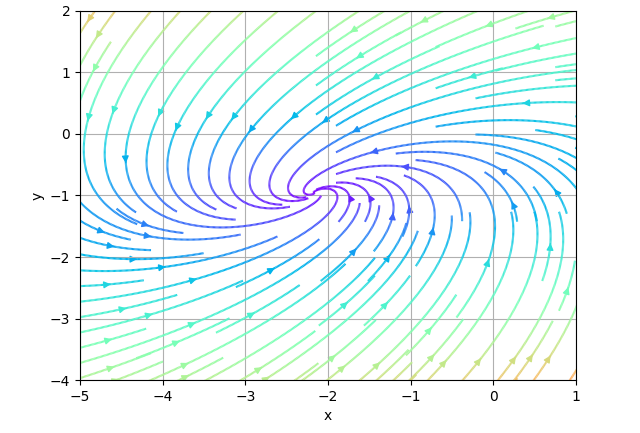
\includegraphics[width=0.7\textwidth]{df_1.png}
    \caption{Фазовый портерт системы в точке $M(-2, -1)$.}
\end{figure}\,\\
$N(4, 2)$:
$$\begin{cases}
        x = u + 4 \\
        y = v + 2
    \end{cases} \  \Rightarrow \quad \begin{cases}
        \dot{u} = \sinh(2(u + 4)(v + 2) - 4(v + 2) - 8) \\
        \dot{v} = \arcsin\left( 4(v + 2)^2 - (u + 4)^2 \right)
    \end{cases} \ \Rightarrow\quad \begin{cases}
        \dot{u} = \sinh(2uv + 4u + 4v) \\
        \dot{v} = \arcsin\left( 4v^2 + 16v - u^2 - 8u \right)
    \end{cases}$$
$$\frac{d}{du}\sinh(2uv + 4u + 4v)\at_{u=0 \atop v=0} = 2(v+2)\cosh(2uv+4u+4v)\at_{u=0 \atop v=0} = 4$$
$$\frac{d}{dv}\sinh(2uv + 4u + 4v)\at_{u=0 \atop v=0} = 2(u+2)\cosh(2uv+4u+4v)\at_{u=0 \atop v=0} = 4$$
$$\frac{d}{du}\arcsin\left( 4v^2 + 16v - u^2 - 8u \right)\at_{u=0 \atop v=0} = \frac{-2u-8}{\sqrt{1 - (4v^2 + 16v - u^2 - 8u)^2}}\at_{u=0 \atop v=0} = -8$$
$$\frac{d}{dv}\arcsin\left( 4v^2 + 16v - u^2 - 8u \right)\at_{u=0 \atop v=0} = \frac{8v+16}{\sqrt{1 - (4v^2 + 16v - u^2 - 8u)^2}}\at_{u=0 \atop v=0} = 16$$
$$\begin{cases}
        \dot{u} = 4u+4v \\
        \dot{v} = -8u+16v
    \end{cases} \ \Rightarrow\quad \begin{vmatrix}
        4-\lambda & 4          \\
        -8        & 16-\lambda
    \end{vmatrix} \ =\ \lambda^{2} - 20 \lambda + 96 = 0 \quad\Rightarrow\quad \lambda_1 = 8,\ \lambda_2 = 12$$
В точке $N(4, 2)$ имеем неустойчивый узел. Найдём собственные векторы, вдоль которых будут проходить фазовые траектории:
$$\text{Имеется матрица } A = \begin{bmatrix}
        4  & 4  \\
        -8 & 16
    \end{bmatrix}. \text{ Найдём собственный вектор } v \text{ для каждого } \lambda, \text{ решив уравнение } (A-I\lambda)v = 0$$
$$\begin{bmatrix}
        -4 & 4 \\
        -8 & 8
    \end{bmatrix}\begin{bmatrix}
        a \\ b
    \end{bmatrix} = \begin{bmatrix}
        0 \\ 0
    \end{bmatrix} \quad\Rightarrow\quad a = b \quad\Rightarrow\quad v_1 = \begin{bmatrix}
        1 \\ 1
    \end{bmatrix}\qquad\qquad\qquad\begin{bmatrix}
        -8 & 4 \\
        -8 & 4
    \end{bmatrix}\begin{bmatrix}
        a \\ b
    \end{bmatrix} = \begin{bmatrix}
        0 \\ 0
    \end{bmatrix} \quad\Rightarrow\quad 2a = b \quad\Rightarrow\quad v_2 = \begin{bmatrix}
        2 \\ 1
    \end{bmatrix}$$
Именно по таким векторам расходится неустойчивый узел. Теперь составим фазовый портрет системы:
\begin{figure}[H]
    \centering 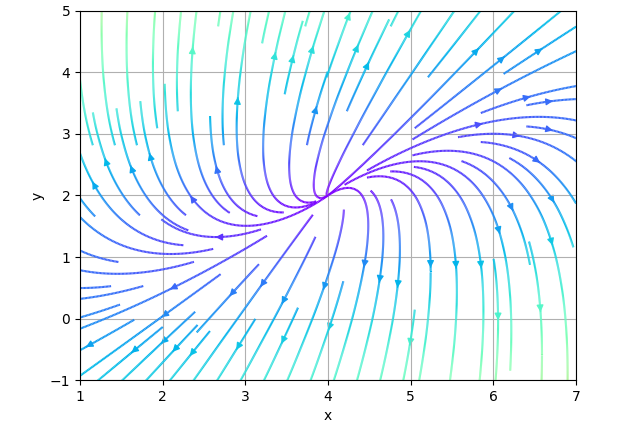
\includegraphics[width=0.7\textwidth]{df_2.png}
    \caption{Фазовый портерт системы в точке $N(4, 2)$.}
\end{figure}

% MARK: Задание №2
\addsection{Задание №2}
\addsubsection{Условие}
Найти общее решение уравнения. Сделать проверку.
$$28.\quad6u_{xx}-7u_{xy}+u_{yy}=0$$
\addsubsection{Решение}
Перед нами дифференциальное уравнение с частными производными второго порядка с двумя независимыми переменными. Для его решения воспользуемся коэффициентами и дискриминантом характеристической формы уравнения:
$$A=6\quad B=-3.5\quad C=1$$
$$\Delta=B^2-AC=3.5^2-6=12.25-6=6.25=2.5^2 > 0 \quad \Rightarrow \text{ уравнение гиперболическое.}$$
$$\frac{dy}{dx}=\frac{B\pm\sqrt{\Delta}}{A} = \frac{-3.5\pm2.5}{6} \quad\Rightarrow\quad \left[\begin{array}{l}
    \dfrac{dy}{dx} = -1 \\
    \vspace{-0.8em} \\
    \dfrac{dy}{dx} = -\dfrac{1}{6}
\end{array}\right. \quad\Rightarrow\quad \left[\begin{array}{l}
    y = -x + C \\
    \vspace{-0.8em} \\
    y = -\dfrac{x}{6} + C
\end{array}\right. \quad\Rightarrow\quad \left[\begin{array}{l}
    C = y + x \\
    \vspace{-0.8em} \\
    C = y + \dfrac{x}{6}
\end{array}\right.$$
Введём замену $U(\gamma, \eta) = u(x, y)$, где $\gamma = y + x$, $\eta = y + \nicefrac{x}{6}$. Найдём каждую из производных $u_{xx},\ u_{xy},\ u_{yy}$, выраженные через $U_{\gamma\gamma},\ U_{\gamma\eta},\ U_{\eta\eta}$:
$$u_x = U_\gamma\gamma_x + U_\eta\eta_x = U_\gamma + \frac{1}{6}U_\eta\qquad\qquad u_y = U_\gamma\gamma_y + U_\eta\eta_y = U_\gamma + U_\eta$$
$$u_{xx} = U_{\gamma\gamma}\gamma_x + U_{\gamma\eta}\eta_x + \frac{1}{6}\left( U_{\eta\gamma}\gamma_x + U_{\eta\eta}\eta_x \right) = U_{\gamma\gamma} + \frac{1}{3}U_{\gamma\eta} + \frac{1}{36}U_{\eta\eta}$$
$$u_{xy} = U_{\gamma\gamma}\gamma_y + U_{\gamma\eta}\eta_y + \frac{1}{6}\left( U_{\eta\gamma}\gamma_y + U_{\eta\eta}\eta_y \right) = U_{\gamma\gamma} + \frac{7}{6}U_{\gamma\eta} + \frac{1}{6}U_{\eta\eta}$$
$$u_{yy} = U_{\gamma\gamma}\gamma_y + U_{\gamma\eta}\eta_y + U_{\eta\gamma}\gamma_y + U_{\eta\eta}\eta_y = U_{\gamma\gamma} + 2U_{\gamma\eta} + U_{\eta\eta}$$
Заменим в исходном уравнении все производные на производные, выраженные через $U$:
$$6\left( U_{\gamma\gamma} + \frac{1}{3}U_{\gamma\eta} + \frac{1}{36}U_{\eta\eta} \right)-7\left( U_{\gamma\gamma} + \frac{7}{6}U_{\gamma\eta} + \frac{1}{6}U_{\eta\eta} \right)+U_{\gamma\gamma} + 2U_{\gamma\eta} + U_{\eta\eta}=0 \quad\Rightarrow$$
$$\Rightarrow\quad\cancel{6U_{\gamma\gamma}} + 2U_{\gamma\eta} + \bcancel{\frac{1}{6}U_{\eta\eta}}-\cancel{7U_{\gamma\gamma}} - \frac{49}{6}U_{\gamma\eta} - \bcancel{\frac{7}{6}U_{\eta\eta}} +\cancel{U_{\gamma\gamma}} + 2U_{\gamma\eta} + \bcancel{U_{\eta\eta}}=0 \quad\Rightarrow\quad - \frac{25}{6} U_{\gamma\eta} = 0 \quad\Rightarrow\quad U_{\gamma\eta} = 0$$\newpage
Проверим, выполнив обратную замену и зная, что $U_{\gamma\eta} = 0$:
$$U_{\gamma\eta} = 0 \quad\Rightarrow\quad \varphi_1(\gamma) + \varphi_2(\eta) = 0 \quad\Rightarrow\quad u = \varphi_1(y+x) + \varphi_2\left( y+\frac{x}{6} \right) = 0$$
$$u_x = \varphi_1(y+x) + \frac{1}{6}\varphi_2\left( y+\frac{x}{6} \right)\qquad\qquad u_y = \varphi_1(y+x) + \varphi_2\left( y+\frac{x}{6} \right)$$
$$u_{xx} = \varphi_1(y+x) + \frac{1}{36}\varphi_2\left( y+\frac{x}{6} \right)\qquad\qquad u_{xy} = \varphi_1(y+x) + \frac{1}{6}\varphi_2\left( y+\frac{x}{6} \right)\qquad\qquad u_{yy} = \varphi_1(y+x) + \varphi_2\left( y+\frac{x}{6} \right)$$
$$6\left( \varphi_1(y+x) + \frac{1}{36}\varphi_2\left( y+\frac{x}{6} \right) \right) -7 \left( \varphi_1(y+x) + \frac{1}{6}\varphi_2\left( y+\frac{x}{6} \right) \right) + \varphi_1(y+x) + \varphi_2\left( y+\frac{x}{6} \right) =$$
$$= \cancel{6\varphi_1(y+x)} + \bcancel{\frac{1}{6}\varphi_2\left( y+\frac{x}{6} \right)} -\cancel{7 \varphi_1(y+x)} - \bcancel{\frac{7}{6}\varphi_2\left( y+\frac{x}{6} \right)} + \cancel{\varphi_1(y+x)} + \bcancel{\varphi_2\left( y+\frac{x}{6} \right)} = 0$$
Действительно, даже с учётом обратной замены равенство $U_{\gamma\eta} = 0$ выполняется. Значит общее решение уравнения найдено верно.


% MARK: Задание №3
\addsection{Задание №3}
\addsubsection{Условие}
Решить первую смешанную задачу на отрезке.
$$\begin{array}{@{}l@{}} 
    28.\ u_{tt} = 9u_{xx},\quad x\in(0, 1),\ t\in(0, \infty); \\
    \quad\ \; u|_{t=0}=10x(1-x),\ u_t|_{t=0}=0,\ u|_{x=0}=u|_{x=1}=0.
\end{array}$$
\addsubsection{Решение}
Предположим решение в виде $u(x, t) = X(x)T(t)$. Подставим его в уравнение в частных производных и получим следующее:
$$X(x)T''(t) = 9X''(x)T(t)$$
Теперь разделим обе части уравнения на $9u(x, t)$:
$$\frac{T''(t)}{9T(t)} = \frac{X''(x)}{X(x)} = -\lambda$$
Таким образом имеем два дифференциальных уравнения:
$$T''(t) + 9\lambda T(t) = 0\qquad\qquad X''(x) + \lambda X(x) = 0$$
Решим второе уравнение для $X(x)$, имея в виду граничные условия $X(0) = X(1) = 0$. Это задача Штурма-Лиувилля, поэтому нетрудно найти собственные значения и собственные функции:
$$\lambda_k = \left( \frac{k\pi}{1} \right) = k^2\pi^2,\qquad X_k(x) = \sin(k\pi x)$$
\vspace{-1.7em}
$$k \in \mathbb{N}$$
Теперь решим уравнение для $T(t)$, подставив найденное собственное значение $\lambda$:
$$T''(t) + 9k^2\pi^2 T(t) = 0\quad\Rightarrow\quad T_k(t) = A_k\cos(3k\pi t) + B_k\sin(3k\pi t)$$
Составим общее решение:
$$u(x, t) = \sum_{k=1}^{\infty} \left( A_k\cos(3k\pi t) + B_k\sin(3k\pi t) \right)\sin(k\pi x)$$
Остаётся найти коэффициенты $A_k$ и $B_k$, используя начальные условия $u(x, 0)=10x(1-x)$ и $u(x, 0) = 0$:
$$u(x, 0) = \sum_{k=1}^{\infty} A_k\sin(k\pi x) = 10x(1-x) \quad\Rightarrow\quad A_k = 2\int_0^1 10x(1-x)\sin(k\pi x)dx \quad\Rightarrow\quad A_k = \frac{40}{k^3\pi^3}\left( 1-(-1)^k \right)$$
$$u_t(x, 0) = \sum_{k=1}^{\infty} 3k\pi B_k\sin(k\pi x) = 0 \quad\Rightarrow\quad B_k = 0 \text{ для всех } k$$
Составим итоговое решение, с учётом того, что $A_k = 0$, если $k$ --- чётное:
$$u(x,t) = \sum_{n=0}^{\infty} \frac{80}{(2n+1)^3\pi^3}\cos\left( 3(2n+1)\pi t \right)\sin\left( (2n+1)\pi x \right)$$
\end{document}